% Options for packages loaded elsewhere
\PassOptionsToPackage{unicode}{hyperref}
\PassOptionsToPackage{hyphens}{url}
%
\documentclass[
]{article}
\usepackage{lmodern}
\usepackage{amssymb,amsmath}
\usepackage{ifxetex,ifluatex}
\ifnum 0\ifxetex 1\fi\ifluatex 1\fi=0 % if pdftex
  \usepackage[T1]{fontenc}
  \usepackage[utf8]{inputenc}
  \usepackage{textcomp} % provide euro and other symbols
\else % if luatex or xetex
  \usepackage{unicode-math}
  \defaultfontfeatures{Scale=MatchLowercase}
  \defaultfontfeatures[\rmfamily]{Ligatures=TeX,Scale=1}
\fi
% Use upquote if available, for straight quotes in verbatim environments
\IfFileExists{upquote.sty}{\usepackage{upquote}}{}
\IfFileExists{microtype.sty}{% use microtype if available
  \usepackage[]{microtype}
  \UseMicrotypeSet[protrusion]{basicmath} % disable protrusion for tt fonts
}{}
\makeatletter
\@ifundefined{KOMAClassName}{% if non-KOMA class
  \IfFileExists{parskip.sty}{%
    \usepackage{parskip}
  }{% else
    \setlength{\parindent}{0pt}
    \setlength{\parskip}{6pt plus 2pt minus 1pt}}
}{% if KOMA class
  \KOMAoptions{parskip=half}}
\makeatother
\usepackage{xcolor}
\IfFileExists{xurl.sty}{\usepackage{xurl}}{} % add URL line breaks if available
\IfFileExists{bookmark.sty}{\usepackage{bookmark}}{\usepackage{hyperref}}
\hypersetup{
  pdftitle={STAT 5825},
  pdfauthor={Ben Stockton},
  hidelinks,
  pdfcreator={LaTeX via pandoc}}
\urlstyle{same} % disable monospaced font for URLs
\usepackage[margin=1in]{geometry}
\usepackage{color}
\usepackage{fancyvrb}
\newcommand{\VerbBar}{|}
\newcommand{\VERB}{\Verb[commandchars=\\\{\}]}
\DefineVerbatimEnvironment{Highlighting}{Verbatim}{commandchars=\\\{\}}
% Add ',fontsize=\small' for more characters per line
\usepackage{framed}
\definecolor{shadecolor}{RGB}{248,248,248}
\newenvironment{Shaded}{\begin{snugshade}}{\end{snugshade}}
\newcommand{\AlertTok}[1]{\textcolor[rgb]{0.94,0.16,0.16}{#1}}
\newcommand{\AnnotationTok}[1]{\textcolor[rgb]{0.56,0.35,0.01}{\textbf{\textit{#1}}}}
\newcommand{\AttributeTok}[1]{\textcolor[rgb]{0.77,0.63,0.00}{#1}}
\newcommand{\BaseNTok}[1]{\textcolor[rgb]{0.00,0.00,0.81}{#1}}
\newcommand{\BuiltInTok}[1]{#1}
\newcommand{\CharTok}[1]{\textcolor[rgb]{0.31,0.60,0.02}{#1}}
\newcommand{\CommentTok}[1]{\textcolor[rgb]{0.56,0.35,0.01}{\textit{#1}}}
\newcommand{\CommentVarTok}[1]{\textcolor[rgb]{0.56,0.35,0.01}{\textbf{\textit{#1}}}}
\newcommand{\ConstantTok}[1]{\textcolor[rgb]{0.00,0.00,0.00}{#1}}
\newcommand{\ControlFlowTok}[1]{\textcolor[rgb]{0.13,0.29,0.53}{\textbf{#1}}}
\newcommand{\DataTypeTok}[1]{\textcolor[rgb]{0.13,0.29,0.53}{#1}}
\newcommand{\DecValTok}[1]{\textcolor[rgb]{0.00,0.00,0.81}{#1}}
\newcommand{\DocumentationTok}[1]{\textcolor[rgb]{0.56,0.35,0.01}{\textbf{\textit{#1}}}}
\newcommand{\ErrorTok}[1]{\textcolor[rgb]{0.64,0.00,0.00}{\textbf{#1}}}
\newcommand{\ExtensionTok}[1]{#1}
\newcommand{\FloatTok}[1]{\textcolor[rgb]{0.00,0.00,0.81}{#1}}
\newcommand{\FunctionTok}[1]{\textcolor[rgb]{0.00,0.00,0.00}{#1}}
\newcommand{\ImportTok}[1]{#1}
\newcommand{\InformationTok}[1]{\textcolor[rgb]{0.56,0.35,0.01}{\textbf{\textit{#1}}}}
\newcommand{\KeywordTok}[1]{\textcolor[rgb]{0.13,0.29,0.53}{\textbf{#1}}}
\newcommand{\NormalTok}[1]{#1}
\newcommand{\OperatorTok}[1]{\textcolor[rgb]{0.81,0.36,0.00}{\textbf{#1}}}
\newcommand{\OtherTok}[1]{\textcolor[rgb]{0.56,0.35,0.01}{#1}}
\newcommand{\PreprocessorTok}[1]{\textcolor[rgb]{0.56,0.35,0.01}{\textit{#1}}}
\newcommand{\RegionMarkerTok}[1]{#1}
\newcommand{\SpecialCharTok}[1]{\textcolor[rgb]{0.00,0.00,0.00}{#1}}
\newcommand{\SpecialStringTok}[1]{\textcolor[rgb]{0.31,0.60,0.02}{#1}}
\newcommand{\StringTok}[1]{\textcolor[rgb]{0.31,0.60,0.02}{#1}}
\newcommand{\VariableTok}[1]{\textcolor[rgb]{0.00,0.00,0.00}{#1}}
\newcommand{\VerbatimStringTok}[1]{\textcolor[rgb]{0.31,0.60,0.02}{#1}}
\newcommand{\WarningTok}[1]{\textcolor[rgb]{0.56,0.35,0.01}{\textbf{\textit{#1}}}}
\usepackage{graphicx,grffile}
\makeatletter
\def\maxwidth{\ifdim\Gin@nat@width>\linewidth\linewidth\else\Gin@nat@width\fi}
\def\maxheight{\ifdim\Gin@nat@height>\textheight\textheight\else\Gin@nat@height\fi}
\makeatother
% Scale images if necessary, so that they will not overflow the page
% margins by default, and it is still possible to overwrite the defaults
% using explicit options in \includegraphics[width, height, ...]{}
\setkeys{Gin}{width=\maxwidth,height=\maxheight,keepaspectratio}
% Set default figure placement to htbp
\makeatletter
\def\fps@figure{htbp}
\makeatother
\setlength{\emergencystretch}{3em} % prevent overfull lines
\providecommand{\tightlist}{%
  \setlength{\itemsep}{0pt}\setlength{\parskip}{0pt}}
\setcounter{secnumdepth}{-\maxdimen} % remove section numbering
\usepackage{float} \floatplacement{figure}{H}

% The following sets up the auto column and subtitle functions from StackOverflow
\usepackage{etoolbox,refcount}
\usepackage{multicol}
\usepackage{titling}

\newcounter{countitems}
\newcounter{nextitemizecount}
\newcommand{\setupcountitems}{%
  \stepcounter{nextitemizecount}%
  \setcounter{countitems}{0}%
  \preto\item{\stepcounter{countitems}}%
}
\makeatletter
\newcommand{\computecountitems}{%
  \edef\@currentlabel{\number\c@countitems}%
  \label{countitems@\number\numexpr\value{nextitemizecount}-1\relax}%
}
\newcommand{\nextitemizecount}{%
  \getrefnumber{countitems@\number\c@nextitemizecount}%
}
\newcommand{\previtemizecount}{%
  \getrefnumber{countitems@\number\numexpr\value{nextitemizecount}-1\relax}%
}
\makeatother    
\newenvironment{AutoMultiColItemize}{%
\ifnumcomp{\nextitemizecount}{>}{3}{\begin{multicols}{2}}{}%
\setupcountitems\begin{itemize}}%
{\end{itemize}%
\unskip\computecountitems\ifnumcomp{\previtemizecount}{>}{3}{\end{multicols}}{}}

\newcommand{\subtitle}[1]{%
  \posttitle{%
    \par\end{center}
    \begin{center}\large#1\end{center}
    \vskip0.5em}%
}

\usepackage[english]{babel}
\setlength{\parindent}{4em}
\setlength{\parskip}{1em}
\renewcommand{\baselinestretch}{1.5}

\usepackage[backend=biber, style=apa, citestyle=authoryear]{biblatex}

\addbibresource{final_project.bib}

\hypersetup{
  colorlinks=true,
  linkcolor=blue,
  filecolor=magenta,
  citecolor=black,
  urlcolor=blue
}

\usepackage{indentfirst}

% \usepackage{apacite}

\title{Investigating Distributed ARIMA Models for Ultra-long \\ Time Series with Twin Cities Traffic Data}
\subtitle{STAT 5825 Final Project}

\author{Ben Stockton}

\begin{document}
\maketitle

\section*{Introduction}

Today's businesses, scientists, and other groups measure more continuous processes more carefully than ever before, yielding multitudes of time series that have many observations that exist over ultra-long time spans. These ultra-long time series challenge traditional modeling methodologies since they inherently violate some of the underlying assumptions, such as constant variance and that the same process generates the entire time series. To provide a new solution to these assumption violations, Wang et al. developed the Distributed ARIMA (DARIMA) framework (\cite*{wang_distributed_2020}). Their new DARIMA method allows the data generating process to vary slowly and continuously over time while still using the entire time series to create a cohesive model that out performs the traditional ARIMA model. DARIMA models provide a clear and convincing advantage over the ARIMA model in forecasting with ultra-long time series and in computation time.

For this project, I used the code provided alongside the DARIMA paper on GitHub (\cite{wang_xqnwang_github_2020}) to replicate the findings on improved performance and decreased computation costs relative to the ARIMA model. For this purpose, I selected the \href{https://archive.ics.uci.edu/ml/datasets/Metro+Interstate+Traffic+Volume}{Metro Interstate Traffic} data set from the UCI Machine Learning Repository\footnote{Accessed here: \href{https://archive.ics.uci.edu/ml/datasets/Metro+Interstate+Traffic+Volume}{https://archive.ics.uci.edu/ml/datasets/Metro+Interstate+Traffic+Volume}} (\cite{hogue_uci_2019}). This data set comprises measurements of hourly traffic volume on I-95 at a point halfway between St. Paul and Minneapolis, hourly temperatures, holiday indicators, as well as a few weather variables\footnote{There appear to be issues with the percipitation measurements. I will discuss this further in the Data section.}. 

To compare the DARIMA model to the traditional ARIMA model, I used the Mean Absolute Scaled Error (MASE) and Mean Scaled Interval Score (MSIS), as were used in the original DARIMA paper (\cite[p.~25]{wang_distributed_2020}). I also followed the lead from Wang et al. to demonstrate both the forecasting and computational efficiency superiority of DARIMA over ARIMA for ultra-long time series, and what model settings yield optimal forecasts, and to investigate some of the properties of those forecasts. (\cite*[p.~21-29]{wang_distributed_2020}).

From my analysis, I was able to replicate some of the results in the DARIMA paper (\cite[p.~21-31]{wang_distributed_2020}), such as the improved overall performance and overall computational efficiency of the DARIMA method compared to the ARIMA method. The DARIMA model produced prediction intervals that were significantly narrower than the ARIMA's while their point forecasts were less distinguishable. The performance of these two models also stabilized quickly at a forecast horizon of $n \approx 100$, where forecasts more than 100 hours (4 days) beyond the end of the observations are the overall mean. Just as important as the forecasting performance benefits, I was able to replicate the massive improvements in computational efficiency of DARIMA over ARIMA when you let the maximum order of the model increase. Finally, as in the DARIMA paper, I also demonstrated that the DARIMA model performs best when each subseries is a length that can be processed by the traditional ARIMA ($n_k \approx 300 \mathrm{~to~}500$) (\cite[p.~31]{wang_distributed_2020}).

The code for the DARIMA framework posted to \href{https://github.com/xqnwang/darima}{GitHub} has not been neatly wrapped into either a Python nor an R package (\cite{wang_xqnwang_github_2020}). At the moment this makes implementing their framework more difficult than usual. The framework requires Spark, so it is ideally employed on a distributed computing system\footnote{A distributed system could probably be set up on the Stats Department cluster, but I haven't taken the introduction "course" to get up to speed on using the cluster. I could have also used Google Cloud Platform or a similar cloud compute engine, but I chose not to pay for the compute time.}. Due to limited access to a distributed system, I set up a single node computer on my personal computer to use Spark for the modeling process. This took a significant amount of time to configure, but once set up the single node works well enough for the demonstration purposes of this project. My time series ($n$ = 48,204) is also significantly shorter than the ultra-long time series ($n$ = 124,171) used for demonstration in the DARIMA paper which decreases the need for a distributed system.

\section*{Discussion of "Distributed ARIMA models for ultra-long time series" (\cite{wang_distributed_2020})}

In the summer of 2020, researchers Xiaoqian Wang, Yanfei Kang, Rob Hyndman, and Feng Li posted their paper, "Distributed ARIMA Models for Ultra-long Time Series" (\cite*{wang_distributed_2020}), to \href{https://arxiv.org/abs/2007.09577}{arXiv.org} in which they develop and demonstrate a methodology for modeling ultra-long time series based on the ARIMA process. Ultra-long time series arise from processes that are observed many, many times over a "long" period of time. Some of the examples discussed by Wang et al. in their paper include hourly electricity demand (which they use to demonstrate their new methodology), daily temperatures over hundreds of years, streaming data that is continuously generated, and stock prices recorded hourly over several years (\cite*[p.~2]{wang_distributed_2020}). 

The motivating hypothesis behind their research is that the data generating process doesn't remain constant over these ultra-long periods, but rather has small, gradual changes which are essentially constant on small enough time scales (\cite*[p.~2]{wang_distributed_2020}). To model this shifting behavior, they developed the DARIMA methodology. The DARIMA methodology splits the ultra-long time series into smaller, easier to model subseries to which ARIMA models are fit. The ARIMA estimates for the subseries are then combined together using a variation of weighted least squares (\cite{zhu_dlsa_2019}). As demonstrated in their paper and my project, this results in models with better accuracy and reduced computation time compared to fitting a single ARIMA model for the entire ultra-long time series.

In their paper, the researchers also discuss alternative methods for modeling ultra-long time series such as discarding early observations, only using later observations for model fitting and forecasting, and the model-free prediction method developed by Das and Politis \footnote{"Predictive inference for locally stationary time series with an application to climate data" (\cite*{das_predictive_2020})} (\cite[p.~2]{wang_distributed_2020}). As mentioned in the paper, these methods have significant computational costs or require an inefficient use of the available data. The DARIMA approach accomplishes more efficient and more accurate modeling using the full data by using distributed computing.

\subsection*{Distributed Computing}

% Pick up with Section 2.1 here.
Distributed computing consists of a network of computing nodes that coordinate with each other to process time consuming computations in a more efficient manner. One particularly common distributed framework is MapReduce (\cite[p.5]{wang_distributed_2020}). In this distributed framework, there typically is one "master" node while the other nodes are "worker" nodes\footnote{In the summer of 2020, the use of this analogy faced renewed scrutiny, albeit under the more odious phrasing as master-slave. The debate over this terminology is ongoing (\cite{eglash_broken_2007}) and several major technology companies and organizations including GitHub, Python, and Twitter have already or are replacing the terminology in their documentation (\cite{landau_tech_2020}).}.  The full data must first be partitioned into independent subsets paired with keys for identification by the "master" node and then passed to the "worker" nodes. The "Map" portion of MapReduce acts as a function by mapping the independent subset-key pairs to the independent outcome-key pairs as calculated by the "worker" nodes. Then the "Reduce" portion of the framework takes the independent outcome-key pairs and then processes them to reduce them down to a final output using an algorithm such as distributed least squares (\cite{zhu_dlsa_2019})(\cite[p.~5]{wang_distributed_2020}). 

There are two primary benefits of distributed computing as discussed by Wang et al. (\cite*[p.~5]{wang_distributed_2020}). The first is the reduced computational time via parallelization, but this also requires more computation overall since the independent results must be merged together rather than a single result being produced by a typical single process computation. The second primary benefit is the ability to scale computation by adding "worker" nodes to the network instead of upgrading the hardware of the existing nodes. A popular technology for working with distributed computing for machine learning and statistical tasks is the Spark system by Apache along with the Hadoop distributed file system (Apache Software \cite{apache_spark}). 

% Section 2.2

As noted by Wang et al., distributed computing does come with limitations for statistical computing. The main limitation is the requirement that the portions of the data that are sent to each "worker" node are independent from all other portions of the data since the individual "worker" nodes cannot communicate with each other to process dependencies (\cite*[p.~7]{wang_distributed_2020}). This is less of a problem when the observations from the data set are independent of each other, such as in the traditional MLR framework. In the DARIMA paper, Wang et al., note that there have been a variety of attempts by researchers to implement forecasting with dependent data on distributed computing, but apparently none have tried to incorporate both distributed computing for the model fitting and for the forecasting as they have described and demonstrated (\cite*[p.~7]{wang_distributed_2020}).

\subsection{ARIMA \& DARIMA Processes and Estimation}
% Section 2.3
% - Background on ARIMA models. I don't think I need to spend too long on this. Mostly focus on their use of auto.arima() and how it works. Be brief. Can discuss and cite the Hyndman paper on the \textbf{forecast} package. (\cite{hyndman_automatic_2008}) (\cite[p.~8-10]{wang_distributed_2020})

As we learned in our course, ARIMA models are fairly flexible and can be used to model time series with both time trends and seasonal trends by adding a differencing component into the ARMA process which combines the AR and MA processes (\cite[p.~99]{shumway_time_2019}). The ARIMA model is specified as ARIMA($p,d,q$) while the seasonal ARIMA is specified as ARIMA($p,d,q) \times (P,D,Q)_s$. The coefficients $p$ and $P$ specify the order of the non-seasonal AR and seasonal AR processes. $q$ and $Q$ specify the order of the non-seasonal MA and seasonal MA processes. $d$ and $D$ specify the order of the differencing, whlie $s$ specifies the seaonal period. The seaonal ARIMA($p,d,q) \times (P,D,Q)_s$ model is given below in eqn. (1):

\begin{equation}
  \Phi_P(B^s)\phi_p(B)(1 - B^s)^D (1 - B)^d x_t = \alpha + \Theta_Q(B^s) \theta_q(B) w_t
\end{equation}

\[
\begin{array}[h]{ll}
  \Phi_P(B^s) = 1 - (\sum_{j = 1}^P \Phi_j B^{sj}) & \Theta_Q(B^s) = 1 + \sum_{j = 1}^Q \Theta_j B^{sj} \\
  \phi_p(B) = 1 - (\sum_{j = 1}^p \phi_j B^j) & \theta_q(B) = 1 + \sum_{j = 1}^q \theta_j B^j
\end{array}
\]

where $\Phi_j, \phi_j, \Theta_j, \theta_j \in (-1,1)$, $B$ is the backshift operator and $w_t$ is a white noise series.

As in our course, Wang et al., use the \textbf{forecast} package's \texttt{auto.arima()} function to fit their overall ARIMA model and the localized ARIMA models for each subseries in the DARIMA framework\footnote{See appendix for a description of the automatic selection algorithm.}. The researchers discuss several issues that come along with the automatic ARIMA fitting in the ultra-long time series domain (\cite[p.~9-10]{wang_distributed_2020}). Among these are:
\begin{itemize}
  \item A constant data generating process is an unrealistic assumption.
  \item ARIMA fitting is a time-consuming process.
  \item Multiple models can be considered in the model refitting process.
  \item Conditional Least Squares (CSS) must be used instead of CSS-ML or ML because it is the least inefficient.
  \item Single node systems may not be able to fit an ARIMA to an ultra-long time series due to resource limitations.
  \item The upper limit on the orders restricts the potential models that could be fit.
\end{itemize} The DARIMA approach uses the ARIMA process locally on each subseries to create a global process to avoid these issues.

% Section 3.1
% - Discuss the way the data is re-structured to enable the Map Reduce to work. Figure 4, Alg 1 \& 2, and the steps around it should be the basis for this discussion. ((\cite[p.~12-15]{wang_distributed_2020}) for the algorithm stuff)
Within MapReduce, the DARIMA modeling framework consists of three steps within "Map": preprocessing, modeling, linear transformation, and then two within "Reduce": estimator combination and forecasting (\cite[p.~13-14]{wang_distributed_2020}). The preprocessing subdivides the the full time series into the $K$ subseries that will be modeled individually. These subseries are passed onto the "worker" nodes. In the modeling step, the "worker" nodes fit the \texttt{auto.arima()} model to the subseries. Then the linear transformation step converts the ARIMA representations of the fitted models into AR($\infty$) representations via invertibility (\cite[p.~16]{wang_distributed_2020}). This completes the "Map" portion of MapReduce. The "Reduce" portion then picks up with the estimate combination step, which uses distributed weighted least squares to combine the subseries' estimates into global estimates in a final AR($\infty$) process. This process is then used for forecasting, completing the DARIMA framework. This process is explained in detail in Figures 3 \& 4 and Algorithms 1 \& 2 in the DARIMA paper (\cite[p.~13-15]{wang_distributed_2020}).

% - Discuss the linear representation of ARIMA models. Why? What are they? ((\cite[p.~16-17]{wang_distributed_2020}) for the ARIMA and ARIMA to AR stuff)

Wang et al. extend invertibility to seasonal ARIMA models by equating the seasonal ARIMA process to an ARMA process by setting $\phi'(B) = \phi(B)\Phi(B)$ and $\theta'(B) = \theta(B) \Theta(B)$ where $\phi(B) = (1 - \sum_{j = 1}^p \phi_j B^j)(1 - B)^d$ and $\Phi(B) = (1 - \sum_{j = 1}^P \Phi_i B^j)(1 - B)^D$ while $\theta(B)$ and $\Theta(B)$ have the typical definitions\footnote{See the appendix for a detailed definition of the ARMA process.} (\cite*[p.~16-17]{wang_distributed_2020}). They characterize this re-expressed process as a ARMA($u,v$) process where $u = p + P$ and $v = q + Q$. Having re-expressed the ARIMA process as an ARMA process, it is a straighforward matter to transform it to the AR($\infty$) representation, where $\pi(B) = \theta'^{-1}(B) \phi'(B)$ to which an intercept and linear trend are added\footnote{The linear trend term takes care of the non-stationarity of the time series. The differencing terms of the ARIMA model are absorbed into $\beta_0$ and $\beta_1$.} (\cite[p.~17]{wang_distributed_2020}). They also take the extra step of defining an approximation AR($p ~ (>> 1)$) to the AR($\infty$) representation 
\begin{equation}
  x_t = \beta_0 + \beta_1 t + \sum_{j = 1}^{\infty} \pi_j x_{t-j} + \epsilon_t \approx \beta_0 + \beta_1 t + \sum_{j = 1}^p \pi_j x_{t-j} + \epsilon_t
\end{equation}
As Wang et al. describe, the AR($p$) representation is used because the distributed least squares approximation method requires that each subseries model must have the same form (\cite*[p.~18]{wang_distributed_2020}). 

% Section 3.2 

The researchers selected Zhu's Distributed Least Squares Approximation (DLSA) for their combination method to estimate the global parameters (\cite[p.~18]{wang_distributed_2020})(\cite{zhu_dlsa_2019}). The DLSA method takes the subseries estimates and calculates a weighted average to create the global estimates. To calculate the global estimates, Wang et al., minimize a global loss function which is the mean of the subseries loss functions. The global estimates for the AR($p$) parameters are a weighted average of the minimizers of the local loss functions and the estimated covariance matrices of the observations of each subseries
\[\tilde{\theta} = \left(\sum_{k = 1}^K T_k \hat{\Sigma}_k^{-1}\right)^{-1}\left(\sum_{k = 1}^K T_k \hat{\Sigma}_k^{-1} \hat{\theta}_k\right).\] 
The global covariance of the observations is estimated as
\[\tilde{\Sigma} = T\left(\sum_{k = 1}^K T_k \hat{\Sigma}_k^{-1}\right)^{-1}\]
where $K$ is the number of subseries, $T_k$ is the length, $\hat{\Sigma}_k$ is the covariance estimate of the observations, and the vector $\hat{\theta}_k$ are the estimates of the AR($p$) process, all for the $k^{th}$ subseries (\cite[p.~18-19]{wang_distributed_2020}).

% Section 3.3 \& 3.4
% - Point forecasts briefly discussed (\cite[p.~19-20]{wang_distributed_2020})
Point forecasts for the DARIMA process are straightforwardly computed using the global estimates of the AR($p$) process, $\tilde{\theta}$ (\cite[p.~19-20]{wang_distributed_2020}). 
\[\hat{y}_T(h) = \tilde{\beta}_0 + \tilde{\beta}_1 (T + h) +
 \begin{cases}
\sum_{j = 1}^p \tilde{\pi}_j y_{T + 1 - j}, & h = 1 \\
\sum_{j = 1}^{h - 1} \tilde{\pi}_j y_{T}(h-j) + \sum_{j = 1}^p \tilde{\pi}_j y_{T + h - j}, & 1 < h < p \\
\sum_{j = 1}^{p} \tilde{\pi}_j y_{T}(h-j), & h \geq p 
\end{cases}\]
The prediction intervals for the DARIMA process are constructed similarly to the prediction intervals for the ARMA process as discussed in Shumway \& Stoffer (\cite*[p.~93-94]{shumway_time_2019}). The prediction interval of the $h$-step ahead forecast is 
\[\hat{y}_T(h) \pm z_{\alpha/2} \tilde{\sigma}_h\]
where the global estimate of the standard error is
\[\tilde{\sigma}^2 = \begin{cases}
  \tilde{\sigma}^2, & h = 1 \\
  \tilde{\sigma}^2(1 + \sum_{j = 1}^{h - 1}\tilde{\theta}_j^2), & h > 1
\end{cases}\]
and $z_{\alpha/2}$ is the $1 - \alpha/2$ quantile of the standard normal distribution (\cite[p.~20-21]{wang_distributed_2020}).

% - Prediction intervals briefly discussed (\cite[p.~20-21]{wang_distributed_2020})

\subsection*{DARIMA Experimentation}
%% After this is Section 4

To demonstrate their new DARIMA framework, the researchers chose to model the publicly available hourly electricity demands of New England\footnote{In this case New England consists of Massachussets, Connecticut, Rhode Island, Vermont, New Hampshire, and Maine} spanning March 1, 2003 to April 30, 2017\footnote{Accessed on \href{https://github.com/camroach87/gefcom2017data}{GitHub} as the GEFCOM2017 data set \cite{roach_camroach87gefcom2017data_2020}} (\cite[p.~21]{wang_distributed_2020}). This data set contains eight time series of electricity demands: one for each of CT, RI, VT, NH, ME, and northeastern, western-central, and southeastern Massachussets. There are also weather and holiday variables included, but these were ignored for the purposes of their paper. The measurements were taken from October 2012 through September 2018 for a total length of 124,171 observations. They chose to split their data such that they would have four months of demands for forecast evaluation. 

In their experimental set up, they chose to have a baseline of 150 subseries for their DARIMA model, resulting in subseries lengths of around 800. They then set parameters along which the subseries models and the comparison ARIMA model should be fit using the \texttt{auto.arima()} function from the \textbf{forecast} package in R (\cite[p.~23]{wang_distributed_2020}). They set max values for $p$ and $q$ at 5, max values for $P$ and $Q$ at 2, the max order ($p + q + P + Q$) at 5, and then fit the DARIMA subseries models with Conditional Least Squares (CSS) with stepwise selection and without parallelization. For their ARIMA model, they fit the model with parallelization enabled which requires disabling stepwise selection. The models are then evaluated using MASE and MSIS (with 95\% prediction intervals)\footnote{See appendix for the formulas for MASE and MSIS.}. Their computing environment differs drastically from mine. They used one "master" node and two "worker" nodes, which each had 32 logical cores, 64 GB RAM, and 160 GB total SSD storage. My set up uses a single computer node with 4 cores, 16 GB RAM, and 256 GB total SSD storage. 

From their modeling, they demonstrate superior performance by the DARIMA method across the board (\cite[p.~25-31]{wang_distributed_2020}). The DARIMA method requires shorter computation times, produces lower MASE and MSIS overall, and produces MASE and MSIS as low or lower than the ARIMA model at nearly all forecast horizons. They also note that the performance gap increases as the forecast horizon increases and as the confidence level of the prediction interval increases from 50\% to 95\%. To conclude their experiment, they also compared the DARIMA method to itself when different numbers of subseries are used and when the maximum model order is changed. They found that the DARIMA method performed best when the number of subseries was between 150 and 200, for a subseries length of around 800. Increasing the maximum model order resulted in marignally higher MASE and MSIS values for the DARIMA model while slightly decreasing them for the ARIMA models. The worst performing DARIMA model out performed the best performing ARIMA model in both metrics. The more significant point here is that increasing the model order from (5,2,5) to (8,4,10) almost doubled the DARIMA computation time from 1.219 minutes to 2.224 minutes while it increased the ARIMA computation time by more than $20\times$ from 4.596 minutes to 117.875 minutes. In my data analysis, I replicated their findings regarding increased computing efficiency and better performance compared to the ARIMA models. % I also tried to extend the method to include ARIMA modeling with exogenous regression variables.

\section*{Data}

For the data analysis portion of the project, I selected the Metro Interstate Traffic data set posted to the \href{https://archive.ics.uci.edu/ml/datasets/Metro+Interstate+Traffic+Volume}{UC Irvine Machine Learning Repository} (\cite*{hogue_uci_2019}). This data set contains a several variables, but we are only concerned with the Traffic Volume. The traffic volume observations in the time series were collected hourly at Minnesota DoT ATR station 301 on I-95, halfway between St. Paul and Minneapolis, and in the westbound direction (traveling from St. Paul to Minneapolis). The hourly observations were collected from October 2, 2012 at 9 a.m. to September 30, 2018 at 11 p.m., $n = 48,204$.

Also included in the data set were variables for the hourly rainfall, hourly snowfall, hourly temperature, holidays, hourly cloud cover, and a verbal description of the weather. There were a few missing values for temperature which could be imputed with the \texttt{ts.clean()} function from the \textbf{forecast} package. The weather data had larger problems. There were only rainfall measurements for around one year of the data set and there were only 63 hours with non-zero snowfall, an impossibility in Minnesota. The 1-hour lag for temperature and the holiday indicator variable could be interesting to use as exogenous variables in an ARIMAX model.

\begin{figure}[ht]
  \begin{center}
    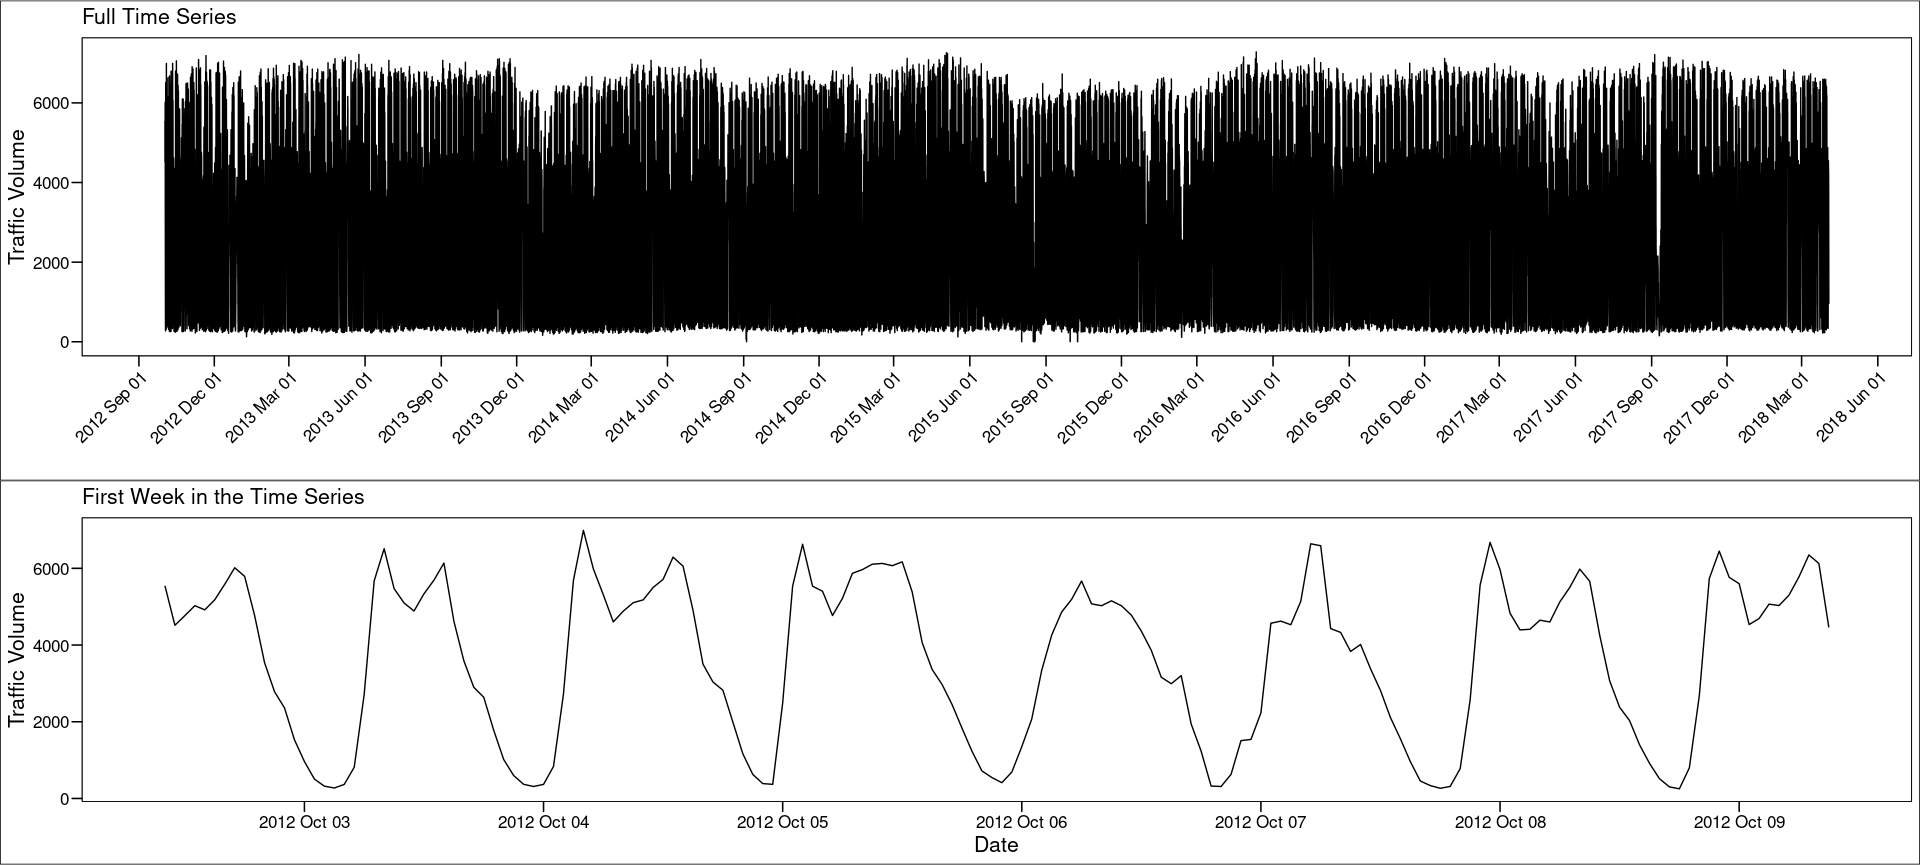
\includegraphics{Plots/full_traffic_ts.png}
    \caption{In the first time series plot, we can see the general behavior of the traffic volume series over the course of six years from October 2012 to April 2018. In the second plot, we can see the behavior of the time series over a single week.}
    \label{fig_ts_plots}
  \end{center}
\end{figure}

In Figure \ref{fig_ts_plots}, we can see the general patterns of the traffic volume time series over the entire span of the data set and in the first week of observations. From the overall plot, we can see that while the time series seems to have the same general process over the course of the six years. Slight variations do appear in the variance at different times along with clear seasonal trends on a 24 hour period with added seasonalities beyond that such as for weeks and seasons/quarters. The plot of the first week in the data set gives us a rough idea of how a given week's traffic volume might vary by the hour. There are clear daily cycles and within each day we can see two peaks for most days at roughly 9 a.m. and 5-6 p.m. This would line up with what we intuitively expect a typical workday's traffic to look like. There is also very little traffic late at night as expected. Overall, this series appears to be an ideal candidate for DARIMA modeling since it is ultra-long and appears to have a slowly varying underlying process.

Before beginning my analysis, I split the full time series into training and testing data sets with the final two months in the testing data set. This gives me a training data set with 46,764 time points and a testing data set with 1,440 time points. 

\section*{Analysis}

Through my analysis and comparison of the ARIMA and DARIMA approaches to ultra-long time series, I replicated the findings of Wang et al. on a different data set and with different hardware supporting both the performance and efficiency improvements found in their research (\cite*[p.21-31]{wang_distributed_2020}). I followed their experimental set up as closely as I could. This includes an overall comparison of the performance and computational efficiency of the two methods, a comparison of the computational efficiencies for different hardware configurations, a sensitivity analysis of DARIMA to $K$ and of the ARIMA and DARIMA models over a selection of model order restrictions. All forecasting performance comparisons for the models are made using the MASE and MSIS metrics. Efficiency comparisons are made using the computation time in seconds. 

As a baseline for the overall comparison, I used the following model settings:
\begin{itemize}
  \item \texttt{max.p = max.q = 5} for both the overall ARIMA and each subseries ARIMA.
  \item \texttt{max.P = max.Q = 2} for both the overall ARIMA and each subseries ARIMA.
  \item \texttt{max.order = 5} for both the overall ARIMA and each subseries ARIMA, where \texttt{max.order} = $p + q + P + Q$.
  \item $K = 150$ subseries for the DARIMA model.
\end{itemize}
The overall ARIMA model was fit with Conditional Least Squares and parallelization instead of stepwise selection. The DARIMA subseries were also fit with Conditional Least Squares, but used stepwise selection instead of parallelization. Model performance is evaluated on the testing data set of the final two months in the time series. Unless otherwise noted, all models are fit using 3 cores.

\begin{figure}[ht]
  \begin{center}
    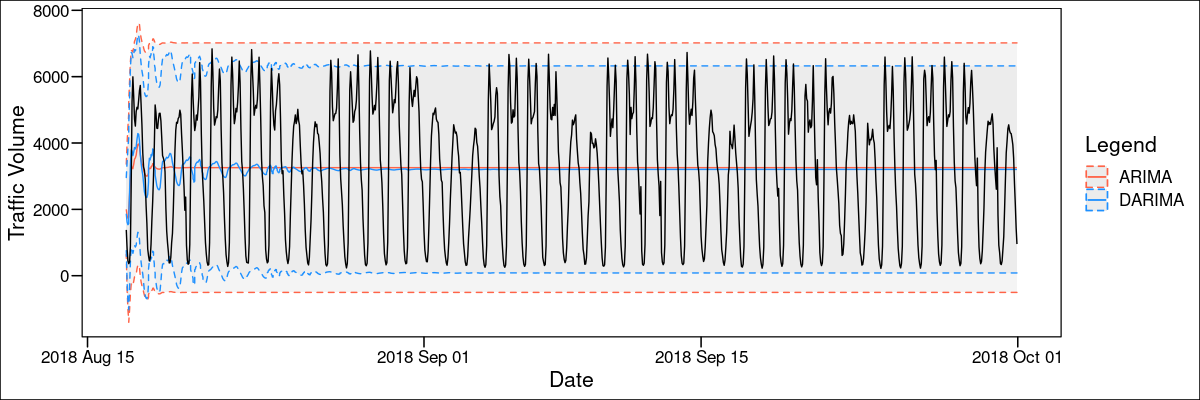
\includegraphics{Plots/arima_darima_forecast.png}
    \caption{This plot compares of the forecasts for the final two months in the data set by the ARIMA model and the DARIMA model. Both prediction bands are at the 95\% level.}
    \label{fig_arima_darima_frct}
  \end{center}
\end{figure}

Overall, the DARIMA method is more computationally efficient and produces better point and interval forecasts than an ARIMA model fit to the traffic data. From Figure \ref{fig_arima_darima_frct}, we can see that the DARIMA forecast has a seasonal trend for longer than the ARIMA forecast, producing better forecasts from roughly $h = 24$ to $h = 168$. For the remainder of the forecast window both processes forecast to the overall mean of the time series. For the whole forecast horizon, DARIMA produces a narrower prediction band compared to the ARIMA process. As in Table \ref{tab-arima-darima-comp}, we can see that the ARIMA model actually produces a better MASE = 1.106, although it's comparable to the DARIMA's MASE = 1.111. The narrower interval produced by the DARIMA model also gives it the lower MSIS of 4.1778 compared to MSIS of 4.7936 for the ARIMA model. The DARIMA model also is more computationally efficient than the ARIMA model, saving over 30 seconds of computation time on this data set. 

\begin{table}
  \begin{center}
    \begin{tabular}[b]{l r r r}
      \hline
      Model & MASE & MSIS & Computation Time \\
      \hline
      ARIMA & \textbf{1.1063} & 4.7936 & 169.56 \\
      DARIMA & 1.1113 & \textbf{4.1778} & \textbf{133.67} \\
      \hline
    \end{tabular}
    \caption{This table shows the overall comparison between ARIMA and DARIMA models at the default model settings. The best scores and time are \textbf{bolded}}
    \label{tab-arima-darima-comp}
  \end{center}
\end{table}

Next, using the overall models, we compare the performances at different forecast horizons in Figure \ref{fig_arima_darima_frct_horizon}. From these plots, we can see that the ARIMA model actually outperforms DARIMA at point estimation for the first 100 or so forecast horizons. Then for the remainder of the horizons, the two models essentially perform identically at point forecasting due to their both forecasting the overall mean. Turning our attention to the prediction intervals, we can see that DARIMA produces markedly more accurate intervals throughout the forecast horizon range. The MSIS of the ARIMA model approaches 5 at $h \approx 100$, while MSIS of the DARIMA model settles around 4 at $h \approx 100$. Again this stabilizing behavior is due to both models forecasting roughly the overall mean as the point forecast beyond $h \approx 100$.

\begin{figure}[ht]
  \begin{center}
    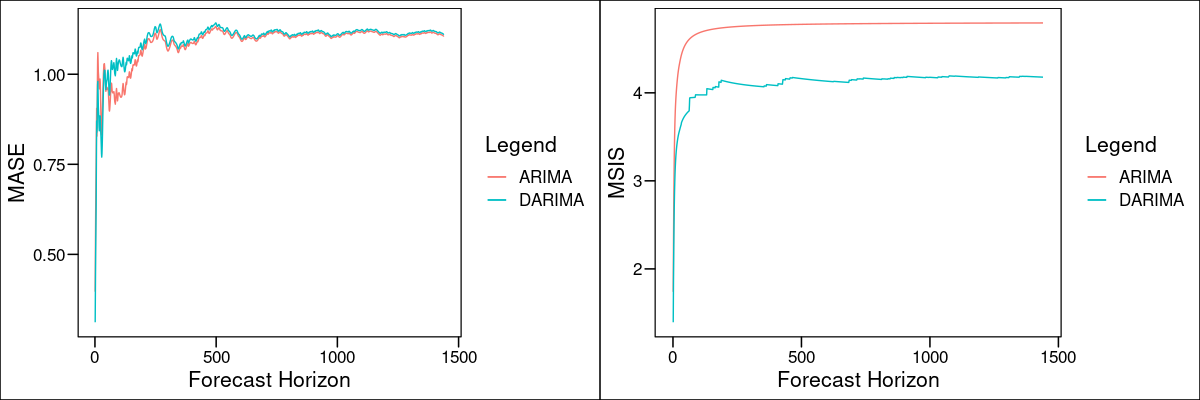
\includegraphics{Plots/arima_darima_forecast_horizon_metrics.png}
    \caption{In these plots we compare the forecast performance metrics at different forecast horizons.}
    \label{fig_arima_darima_frct_horizon}
  \end{center}
\end{figure}

We are also interested in how the computational set up alters the computation time for each model. While this comparison is largely relevant to personal laptops, it is useful to see that the distributed computing and parallelization provide computational efficiency benefits even on this scale. In the DARIMA paper, the researchers found that the computational times decay exponentially as the number of cores increases from 1 to 64\footnote{For ARIMA, time drops from 12+ min to 5 min. For DARIMA, time drops from 10 min to <1 min.} (\cite[p.~30]{wang_distributed_2020}). Table \ref{tab-arima-darima-comp-cores} shows the computational times for each model when run on 1, 2, and 3 cores\footnote{Most personal laptops and personal desktops have 4 to 8 total cores.}. The efficiency gains are far less dramatic for my analysis, in part because of my hardware and in part because my time series is a third of the length of the DARIMA group's time series. Even in the restricted range of possible cores, we see that increasing from 1 to 3 cores saved nearly a minute for fitting and forecasting with the ARIMA model and over a minute when doing the same with the DARIMA model. 

\begin{table}[h]
  \begin{center}
    \begin{tabular}{l | r r}
      \hline
      Model Type & Number of Cores & Computation Time (s) \\
      \hline
      ARIMA & 1 & 240.90 \\
      ARIMA & 2 & 215.28 \\
      ARIMA & 3 & 169.56 \\
      DARIMA & 1 & 200.70 \\
      DARIMA & 2 & 138.18 \\
      DARIMA & 3 & \textbf{133.6678} \\
      \hline
    \end{tabular}
    \caption{The computation times of the DARIMA models are better than those of the ARIMA models at each respective core count. The best time is \textbf{bolded}.}
    \label{tab-arima-darima-comp-cores}
  \end{center}
\end{table}

When we let the settings used to determine our DARIMA model vary, we see that performance and computational efficiency differ drastically. When the DARIMA research group conducted their sensitivity analysis, they varied the number of subseries $K$ of the DARIMA model and the max order of the ARIMA and DARIMA models (\cite[p.30]{wang_distributed_2020}). Their methodology for the sensitivity analysis was roughly analogous to hyperparameter tuning with grid search for a machine learning model. They found that their DARIMA model produces the best forecasts when $K \approx 100$ for both MSIS and MASE with much higher values for each forecast metric at low and high values of $K$. Their conclusion is that the DARIMA method performs best when the ARIMA subseries are given substantial amounts of data, but small enough segments that the underlying data generating process remains constant on that sub-interval. Their comparison of the ARIMA and DARIMA models under different maximum orders, provided some of the most striking conclusions in the paper (\cite[p.~31]{wang_distributed_2020}): DARIMA's computational cost only went up linearly while ARIMA's grew exponentially, and regardless of the maximum order DARIMA always outperformed ARIMA.

In my analysis, I replicated both sensitivity analysis results. With the maximum orders of the models, the DARIMA method ultimately selected models on the order of 5-7 or some combination of models that produced roughly equivalent forecasts since the performance metrics stabilized after increasing the max order to 7 as is seen in Table \ref{tab-max-order}. Increasing the max order beyond 7 offered more models for DARIMA to check, but it settled quickly for the models on the order of 7. Note that the computational times increase from 137.90 seconds to only 207.08 seconds for the DARIMA method. By comparison when we fit the ARIMA models, the algorithm must search through all possible models since parallelization is enabled and not stepwise selection. This results in exponentially increasing computation times from 222 seconds to over two hours. More importantly, I have also found that all of the DARIMA models outperform the best ARIMA model, and that all of the DARIMA models were fit more quickly than the quickest ARIMA model. 

\begin{table}
  \begin{center}
    \begin{tabular}[b]{l| l c c c}
      \hline
      Max. Order & Model & MASE & MSIS & Computational Time (s) \\
      \hline
      (5,5,2,2,5) & ARIMA & 1.1469 & 4.9698 & 222.56 \\
       & DARIMA & \textbf{1.1113} & \textbf{4.1778} & \textbf{137.90} \\
      (6,6,2,2,7) & ARIMA & 1.1483 & 4.9442 & 519.72 \\
       & DARIMA & \textbf{1.1114} & \textbf{4.1802} & \textbf{172.95} \\
      (6,6,3,3,10) & ARIMA & 1.1471 & 4.8996 & 2724.48 \\
       & DARIMA & \textbf{1.1120} & \textbf{4.1834} & \textbf{216.65} \\
      (8,8,4,4,10) & ARIMA & 1.1471 & 4.8996 & 6475.86 \\
       & DARIMA & \textbf{1.1122} & \textbf{4.1883} & \textbf{207.08} \\
      \hline
    \end{tabular}
    \caption{This table contains the forecasting metrics and computational times for the ARIMA and DARIMA methods. The "Max. Order" column indicates the maximum order for auto.arima() function at the local level for DARIMA and overall for ARIMA. The tuple is (\texttt{max.p}, \texttt{max.q}, \texttt{max.P}, \texttt{max.Q}, \texttt{max.order}). The best score and time at each order is \textbf{bolded}.}
    \label{tab-max-order}
  \end{center}
\end{table}

In the second part of their sensitivity analysis, Wang et al. found the sweet spot for the DARIMA model with their data set (\cite*[p.~30]{wang_distributed_2020}). Based on their analysis, it seems like the optimal subseries length is around 700 to 800 for the GEFCOM2017 data set. From my analysis, I can see that DARIMA performs best with subseries with an approximate length of 300 to 400. When $K$ is small, the DARIMA behaves more like an ARIMA model, so its forecasts are not optimal. When $K$ is large, the persistence of the periodic behavior in the forecasts is extended, but the forecasts become slightly shifted compared to the true period, resulting in much higher MSIS but lower MASE in Figures \ref{fig_darima_frct_mets} and \ref{fig_darima_k150_k600}.

\begin{figure}[ht]
  \begin{center}
    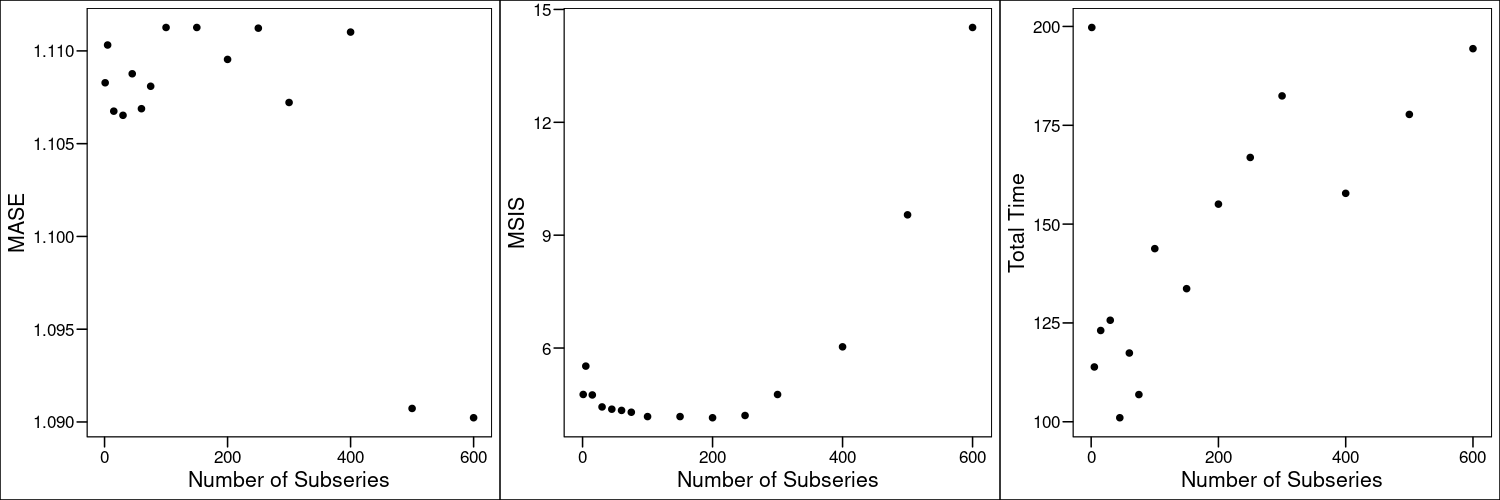
\includegraphics{Plots/darima_metrics_by_n_par.png}
    \caption{The first two plots from left to right show how the DARIMA model performs when different numbers of subseries $K$ are selected. The third plot shows the increase in computation time as the number of subseries increases.}
    \label{fig_darima_frct_mets}
  \end{center}
\end{figure}

Going beyond the results presented in the DARIMA paper, I also compared the computational time for the various numbers of subseries and found that the time increased linearly as the number of subseries increased. The exception to that rule is when $K = 1$, or when fitting a single ARIMA to the whole data set. Interestingly, the computational time drops immediately when $K = 2$. The best computational time is achieved around $K = 75$. In my case, that would yield subseries with an approximate length of 600. 

\section*{Discussion}

The distributed computing approach to ultra-long time series forecasting seems to be very fruitful considering the results Wang et al. found in their research and my results for this project (\cite*{wang_distributed_2020}). The distributed approach offers significant forecasting improvements along with computational efficiency gains, especially when the model orders are allowed to increase. One possible criticism of the DARIMA paper is the use of parallelization instead of stepwise selection for the ARIMA models when comparing the computational times. This would seem to stack the deck in favor of DARIMA having a more efficient performance. It would be of interest to see more explanation behind this decision from the researchers.

Through my analysis, I was able to create a a suitable forecast for up to 100-steps ahead with the DARIMA model while I was only able to create a suitable forecast for up to 24-steps ahead with the ARIMA model. Beyond those forecast horizons, the models largely fit to the overall mean. In this particular context, DARIMA provides useful forecasts for roughly 4 times longer than an ARIMA model. The rate of decay to the overall mean in the DARIMA forecast is also much slower than the ARIMA, not settling at the mean until just over the two week or the 336-step forecast. However, the forecasts between the 100-step forecast and 336-step forecast vary only slightly from the mean and provide only marginal value.

The tendency to forecast the mean is a stark contrast compared to the forecasts produced in the DARIMA paper (\cite[p.~28]{wang_distributed_2020}). Their forecasts of both the ARIMA and DARIMA models have a periodic behavior throughout the forecast horizon, yielding better forecasts compared to mine when $K = 150$. When I let the number of subseries $K$ increase, the forecast's periodic behavior lasts longer into the forecast horizon, as in Figure \ref{fig_darima_k150_k600}. The more persistent periodic behavior leads to the lower MASE values when $K$ is large as we saw in Table \ref{fig_darima_frct_mets}. However, we can also see that the cycles of the prediction intervals are slightly shifted relative to the cycles in the observations, which leads to the higher MSIS from Table \ref{fig_darima_frct_mets}. One possible explanation is that my time series requires a different approach such as differencing by the higher order seasonal trends (weekly, monthly, quarterly, etc) beyond the 24 hour period. However, the GEFCOM2017 data set used by Wang et al. should also have these same issues of higher order seasonalities and they did not report performing any additional data processing in the DARIMA paper\footnote{No additional processing is in their code posted to GitHub either (\cite{wang_xqnwang_github_2020}).} (\cite*{wang_distributed_2020}).

\begin{figure}[ht]
  \begin{center}
    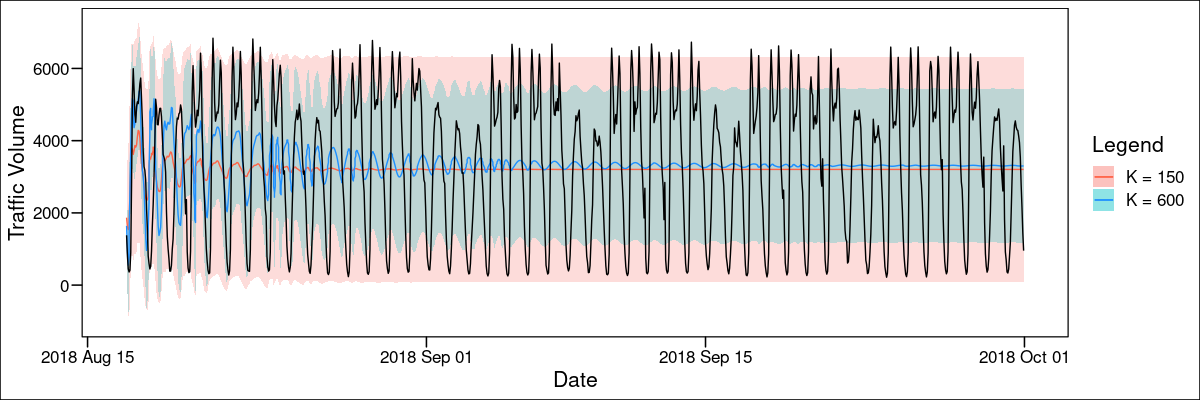
\includegraphics{Plots/darima_k_150_k_600.png}
    \caption{This plot depicts the forecasts for the DARIMA model when the number of subseries $K = 150$ and when $K = 600$. The red band is the 95\% prediction interval for the $K = 150$ DARIMA, while the blue band is the 95\% prediction interval for the $K = 600$ DARIMA.}
    \label{fig_darima_k150_k600}
  \end{center}
\end{figure}

While I was able to replicate most of the findings of the DARIMA research group, I did have significant difficulty setting up my computing environment. This is likely not a significant hurdle in an industrial or academic environment where there are experts with experience using distributed systems. For individuals working on small projects or competitions, this set up hurdle is likely too large to make the DARIMA approach feasible in its current implementation\footnote{Unfortunately, as a result, the code submitted along with this project will not run on a graders computer.}.

A possible alternative to implementing the DARIMA framework would be to use parallelization on a single node computer without Spark. In this context, the ultra-long time series is still partitioned as before, and each subseries model is fit in parallel to produce local estimates that could be combined using a similar (or possibly the same) Reduce framework as developed in the DARIMA paper. The central drawback to using parallelization instead of distributed computing is the loss of "horizontal scalability", or the ability to add additional nodes instead of upgrading hardware, as it was described by Wang et al. (\cite*[p.~5]{wang_distributed_2020}). Instead the hardware of the single computer must be upgraded to add cores to the CPU or the processing could be offloaded to a GPU that has many more cores than a CPU. The main benefit is the more simple implementation that could likely be wrapped up in an R package by using the \texttt{parallel}, \texttt{doparallel}, and \texttt{foreach} packages or in Python with Python equivalent packages. If the DARIMA framework were packaged neatly for either Python or R, it would be a useful method to use for introducing statistical distributed computing in coursework as it combines a relatively simple to state overall problem, an intuitive explanation for how distributed computing would improve the modeling, the relative speed with which the distributed computations can be run on even low-end hardware, but with the added complication of having dependencies between the observations. 

As a next step, it would useful to extend regression models with ARMA errors or ARIMAX models to the DARIMA framework. The code provided by Wang et al. is nearly set up for this extension, but I did not have time to figure out how to use the DLSA approach to combine the local $\beta_j$ estimates to create the global model. Another issue I encountered trying to extend the DARIMA framework is uncertainty regarding how to evaluate the standard error of the forecasts. The extension to regression models with ARMA errors seems like the most direct approach since the \texttt{auto.arima()} function fits regression models with ARMA errors. Alternatively, one could fit local regressions and then run \texttt{auto.arima()} function on the residuals to create local ARMA processes for each of the subseries, then use DLSA on the local regression estimates and the ARMA estimates separately\footnote{This is essentially the same as using \texttt{auto.arima()} with \texttt{xreg} regressors.}. 

\section*{Conclusion}

In conclusion, the DARIMA framework developed by Wang et al. provides a useful structure for creating an ARIMA-type model that violates fewer assumptions, creates better forecasts, and is more computationally efficient than more traditional methods (\cite*{wang_distributed_2020}). There are a few interesting next steps to go with this style of modeling. One would be an extension to using exogenous variables for regression with DARIMA errors or DARIMAX. Another interesting extension would be to compare the performance of this framework to some of the other distributed or modern frameworks mentioned by Wang et al. in their background section (\cite*[p.~7]{wang_distributed_2020}). 

In my analysis of hourly traffic data collected over six years, I replicated the findings of the DARIMA paper with regards to improved computational efficiency and improved forecasting over ARIMA models for ultra-long time series. Being able to replicate their results on low-power hardware indicates that the DARIMA framework would be useful even in small-scale projects. I also used their sensitivity analysis procedure to determine the settings under which DARIMA performs best and to show the stark divide in computational times for ARIMA and DARIMA when the model order is allowed to increase modestly. This led to the interesting result of the shorter subseries DARIMA (large $K$), producing forecasts with a more persistent seasonality. 

\printbibliography
% \bibliographystyle{apacite}
% \bibliography{final_project}

\pagebreak
\section{Appendix}

\subsubsection*{Invertibility of ARMA Processes}
The invertibility of ARMA processes is well-established and we covered the topic in our course and in \textit{Time Series: A Data Analysis Approach Using R} (\cite*[p.~73]{shumway_time_2019}). The time series $x_t$ is invertible if the roots of its $\phi(B)$ polynomial have modulus greater than 1. In the ARMA context this means that the process:
\begin{equation}
  \phi(B)(x_t - \mu) = \theta(B)w_t
\end{equation}
can be expressed in the AR($\infty$) representation 
\begin{equation}
w_t = \sum_{j = 0}^{\infty} \pi_j x_{t-j} = \pi(B) x_t = \theta^{-1}(B)\phi(B)x_t
\end{equation}
where $\sum_{j = 0}^{\infty} \pi^2 < \infty$.

\subsection*{Automatic ARIMA Selection Algorithm}
As described by Hyndman, the algorithm for selecting the most appropriate ARIMA order follows two main steps (\cite[p.~10-12]{hyndman_automatic_2008}). The first step is using unit root tests to determine the order of the differencing\footnote{KPSS unit root test for the non-seasonal differencing and Canova-Hansen unit root test for the seasonal differencing. $D$ is selected before $d$.}. The second step in the automatic selection is to use an information criterion (AIC, AICc, BIC) to traverse the space of possible models in a stepwise manner to select the best model given the upper limits on the orders of $p, q, P$ and $Q$. At each step, we select the model with the lowest information criterion to move forward with and consider the next possible set of models with $\pm 1$ to each of the $p, q, P$ and $Q$ parameters. When no models can beat our current selection, the process ends. 

\subsection*{Formulas Evaluation Metrics}

\[MASE = \frac{\frac{1}{H} \sum_{t = T + 1}^{T+H} |y_t - \hat{y}_{t|T}|}{\frac{1}{T-m}\sum_{t = m+1}^T |y_t - y_{t-m}|}\]

\[MSIS = \frac{\frac{1}{H}\sum_{t = T+1}^{T+H}\left[(U_{t|T} - L_{t|T}) + \frac{2}{\alpha}(L_{t|T} - y_t)I(y_t < L_{t|T}) + \frac{2}{\alpha}(y_t - U_{t|T})I(y_t > U_{t|T})\right]}{\frac{1}{T-m}\sum_{t = m+1}^T |y_t - y_{t-m}|}\]

\end{document}

